\begin{frame}{Introduction}
  \section{Introduction}
  \begin{spacing}{1.2}
  \begin{columns}[T] 
    \begin{column}{0.5\textwidth}

 \begin{itemize}
    \item  Köppen climate classification: tundra (ET) and ice cap (EF). 
    \item Defined as the area north of the Arctic Circle ($66^{\circ}33'$ N).
    \item Sub-regions:
    \begin{itemize}
      \item Arctic maritime region vs. Arctic continental region 
      \item High Arctic vs. Low Arctic
    \end{itemize}
    \item Drainage from river systems (Mackenzie, Lena, Yenisey, Ob, etc.)
    \item The cryosphere (glaciers, permafrost, snow, and sea ice)
   \end{itemize}

    \end{column}
    \begin{column}{0.5\textwidth} 
      \begin{figure}
    \centering
    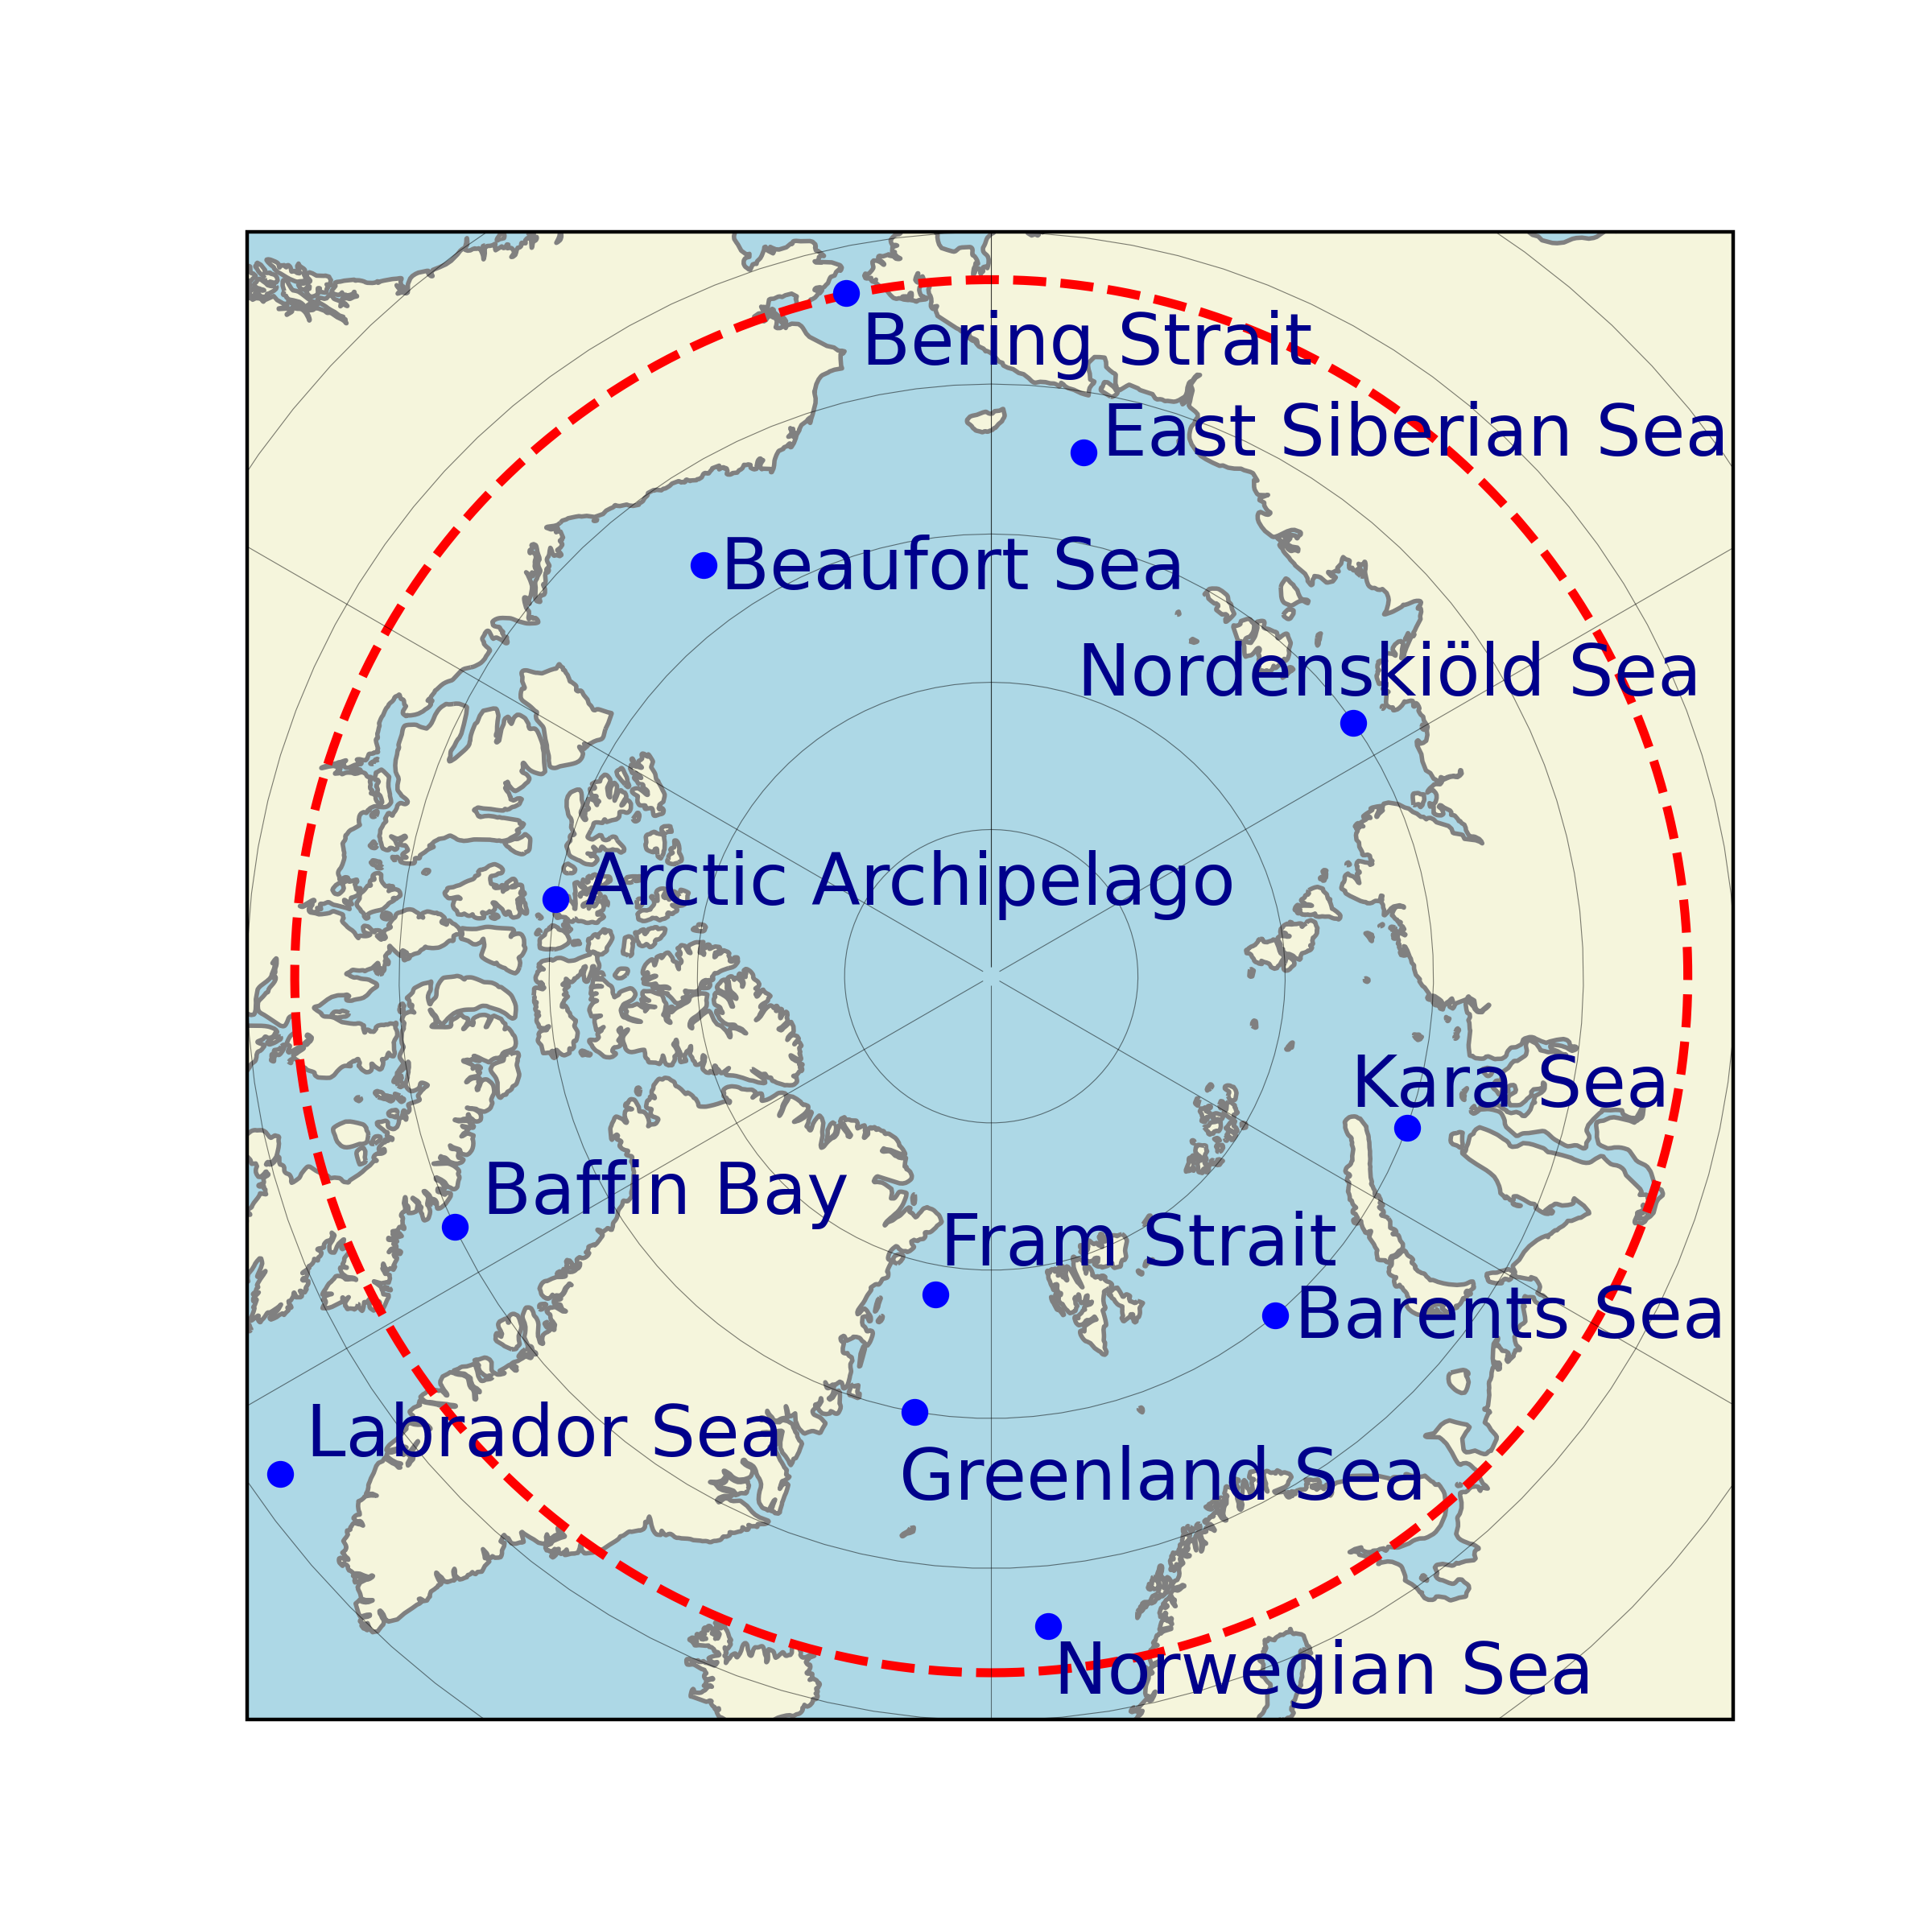
\includegraphics[width=\textwidth]{Figures/map.png}
    \caption{A map of the Arctic.}
  \end{figure}
    \end{column}
  \end{columns}
  \end{spacing}
\end{frame}



\begin{frame}{The regional climate -- Annual Means}
    \section{The regional climate}
    \begin{figure}
        \begin{subfigure}[b]{0.49\textwidth}
            \centering
            
\includegraphics[height=0.4\textheight,keepaspectratio]{Figures/TotalPrecipitation_annual.pdf}
            \caption{Average daily Precipitation}
        \end{subfigure}
        \hfill
        \begin{subfigure}[b]{0.49\textwidth}
            \centering
            
\includegraphics[height=0.4\textheight,keepaspectratio]{Figures/SeaLevelPressure_annual.pdf}
            \caption{Sea Level Pressure}
        \end{subfigure}
        \caption{Annual mean sea level pressure  and total monthly precipitation (2015--2025). All the data was downloaded through the \citet{copernicus_climate_change_service_era5_2023}.}
    \end{figure}
\end{frame}

\begin{frame}{Monthly Means}
    \begin{figure}
        \begin{subfigure}[b]{0.49\textwidth}
            \centering
            
\includegraphics[height=0.4\textheight,keepaspectratio]{Figures/SeaLevelPressure_mean_DJF.pdf}
            \caption{Sea Level Pressure}
        \end{subfigure}
        \hfill
        \begin{subfigure}[b]{0.49\textwidth}
            \centering
            
\includegraphics[height=0.4\textheight,keepaspectratio]{Figures/SeaLevelPressure_mean_JJA.pdf}
            \caption{Sea Level Pressure}
        \end{subfigure}
        \caption{Monthly mean sea level pressure  (2015--2025).}
    \end{figure}
\end{frame}

\begin{frame}{Winter conditions}
    \begin{figure}
        \begin{subfigure}[b]{0.49\textwidth}
            \centering
            
\includegraphics[height=0.4\textheight,keepaspectratio]{Figures/Temperature_mean_DJF.pdf}
            \caption{Temperature}
        \end{subfigure}
        \hfill
        \begin{subfigure}[b]{0.49\textwidth}
            \centering
            
\includegraphics[height=0.4\textheight,keepaspectratio]{Figures/SeaIce_mean_DJF.pdf}
            \caption{Sea Ice}
        \end{subfigure}
    \end{figure}
\end{frame}

\begin{frame}{Spring conditions}
    \begin{figure}
        \begin{subfigure}[b]{0.49\textwidth}
            \centering
            
\includegraphics[height=0.4\textheight,keepaspectratio]{Figures/Temperature_mean_MAM.pdf}
            \caption{Temperature}
        \end{subfigure}
        \hfill
        \begin{subfigure}[b]{0.49\textwidth}
            \centering
            
\includegraphics[height=0.4\textheight,keepaspectratio]{Figures/SeaIce_mean_MAM.pdf}
            \caption{Sea Ice}
        \end{subfigure}
    \end{figure}
\end{frame}

\begin{frame}{Summer conditions}
    \begin{figure}
        \begin{subfigure}[b]{0.49\textwidth}
            \centering
            
\includegraphics[height=0.4\textheight,keepaspectratio]{Figures/Temperature_mean_JJA.pdf}
            \caption{Temperature}
        \end{subfigure}
        \hfill
        \begin{subfigure}[b]{0.49\textwidth}
            \centering
            
\includegraphics[height=0.4\textheight,keepaspectratio]{Figures/SeaIce_mean_JJA.pdf}
            \caption{Sea Ice}
        \end{subfigure}
    \end{figure}
\end{frame}

\begin{frame}{Autumn conditions}
    \begin{figure}
        \begin{subfigure}[b]{0.49\textwidth}
            \centering
            
\includegraphics[height=0.4\textheight,keepaspectratio]{Figures/Temperature_mean_SON.pdf}
            \caption{Temperature}
        \end{subfigure}
        \hfill
        \begin{subfigure}[b]{0.49\textwidth}
            \centering
            
\includegraphics[height=0.4\textheight,keepaspectratio]{Figures/SeaIce_mean_SON.pdf}
            \caption{Sea Ice}
        \end{subfigure}
    \end{figure}
\end{frame}

\begin{frame}{The general circulation -- The Atmosphere}
  \begin{spacing}{1.2} 
  \section{The general circulation}
  \begin{columns}[T] 
    \begin{column}{0.6\textwidth} 

\begin{itemize}
    \item The Arctic atmosphere and large-scale circulation:
    \begin{itemize}
         \item Polar cell subsidizes air in the North Pole, creating a high-pressure system.
         \item Dry, desert-like climate (subsidence and with inversion). 
    \end{itemize}
    \item Arctic Oscillation (AO) measures pressure differences between the Arctic and mid-latitudes. Stronger during the winter.
    \item Easterlies
    \item Extratropical cyclones \citep{serreze2014}.
  \end{itemize}

    \end{column}
    \begin{column}{0.4\textwidth} 
      \begin{figure}
        \centering
        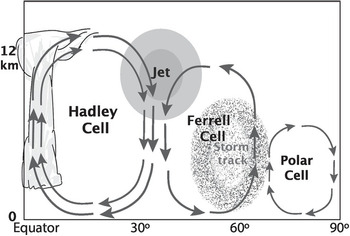
\includegraphics[width=0.8\textwidth]{Figures/polar-cell.jpg}
        \caption{The polar cell illustrated \citep{Trenberth_2022}}
      \end{figure}
      \begin{figure}
        
\includegraphics[width=0.8\textwidth]{Figures/SurfaceWind_annual.pdf}
        \caption{Surface winds (2015--2025)}
      \end{figure}
    \end{column}
  \end{columns}
  \end{spacing}
\end{frame}


\begin{frame}{The Ocean}
  \begin{spacing}{1.2} 
  \begin{columns}[T] 
    \begin{column}{0.6\textwidth} 
      \begin{itemize}

    \item The Arctic Ocean is semi-isolated, the Fram Strait.
    \item Arctic part and the Atlantic meridional overturning circulation:
    \begin{enumerate}
      \item Gulf stream moves East, and then North $\longrightarrow$ Norwegian Current 
      \item Heat flux from ocean to atmosphere..
      \item River discharge lowers salinity.
      \item Brine rejection increases salinity and density, causing water to sink.
      \item Water exits as cold, less saline North Atlantic Deep Water (NADW).
    \end{enumerate}
    \item Southward flow through the East Greenland and Labrador Currents.
    \item Sea ice rotates as a high in the Beaufort Gyre.

    
  \end{itemize}
    \end{column}
    \begin{column}{0.4\textwidth} 
      \begin{figure}
        \centering
        
\includegraphics[width=\textwidth]{Figures/SeaSurfaceTemperature_annual.pdf}
        \caption{Sea Surface Temperature (2015--2025)}
      \end{figure}
    \end{column}
  \end{columns}
  \end{spacing}
\end{frame}

